\documentclass[
        a4paper,     % Format A4
        titlepage,   % mit Titelseite
        twoside,     % zweiseitig
        parskip      % mit Durchschuss
                                 % (= Abstand zwischen Absätzen, statt Einrückung)
        ]{scrartcl} % KOMA-Script Grundklasse     texdoc scrguide

\usepackage[USenglish]{babel}
\usepackage[T1]{fontenc}          % Schriftkodierung mit Umlauten
\usepackage{textcomp,amsmath}     % Mathezeichen etc.
\usepackage{graphicx}             % Graphiken einbinden
\usepackage[utf8]{inputenc}				% direkte Eingabe von Umlauten & Co. (Vorsicht: Encoding im Editor muss auch UTF-8 sein!)

% bibtex
\usepackage{url}
\bibliographystyle{plaindin}      % BibTeX Styles nach Norm DIN 1505

\renewenvironment{abstract}
% https://tex.stackexchange.com/questions/151583/how-to-adjust-the-width-of-abstract
 {\small
  \begin{center}
  \bfseries \abstractname\vspace{-.6em}\vspace{0pt}
  \end{center}
  \list{}{
    \setlength{\leftmargin}{.6cm}%
    \setlength{\rightmargin}{\leftmargin}%
  }%
  \item\relax}
 {\endlist}

\titlehead{

\includegraphics{hpi_logo_cmyk_wb_sl2}
} \subject{Bachelor Thesis}
\title{Feature Extraction for Business Entity Linking in Newspaper Articles
\\ \bigskip 
\large{Merkmalsextraktion zur Unternehmenserkennung in Zeitungsartikeln}}
\author{Jonathan Janetzki\\{\small{\url{jonathan.janetzki@student.hpi.de}}}}
\date{July 21, 2017}
\publishers{
Information Systems Group\\
~\\
\textbf{Supervisors}\\
Prof. Dr. Felix Naumann\\
Toni Grütze\\
Michael Loster}


\pagestyle{headings}    % Seitenstil mit Kapitelüberschriften in der Kopfzeile


\begin{document}

\maketitle
\newpage



% Und: Text \dots
\begin{abstract}

\end{abstract}
\newpage

{\small\tableofcontents}
\newpage

\section{Ambiguous Business Aliases}
e.g., Aldi (Aldi Nord / Aldi Süd)

\section{Related Work}
\subsection{Alias generation to improve company recognition in text}
(Alexander Immer)
\subsection{The CohEEL project}

\section{Text Mining Pipeline}
Preprocesing on Wikipedia dump\\
Explanation of jobs and their runtimes\\
Tools: Stanford CoreNLP (Tokenizer), Apache Lucene (Stemmer)\\
Data structures: Trie (for alias recognition)\\

\subsection{Overview}
see Fig. \ref{fig:job_dependencies}
\begin{figure}[ht]
	\centering
  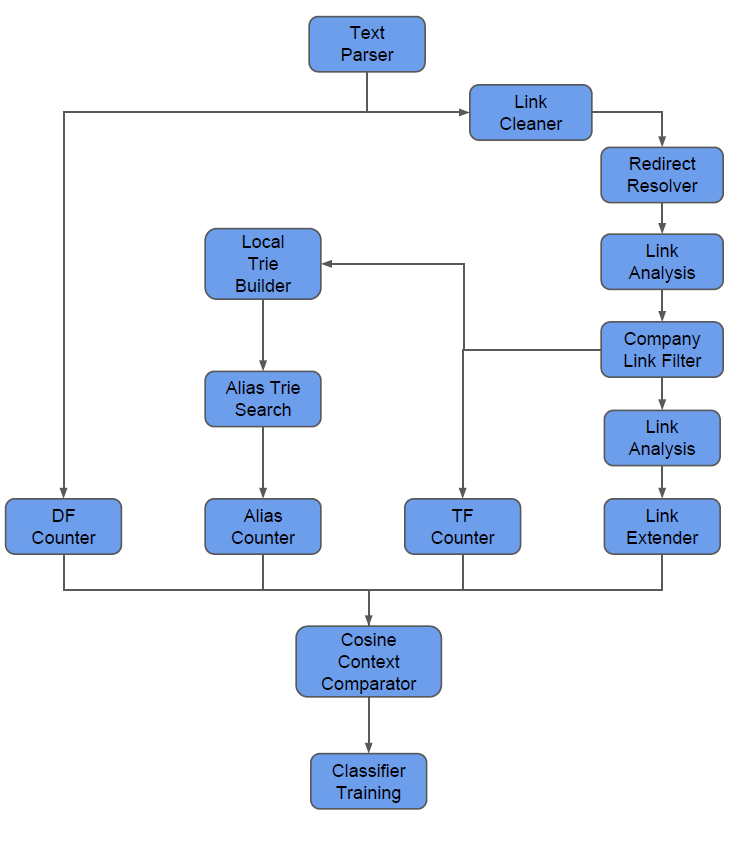
\includegraphics[width=0.7\textwidth]{job_dependencies.png}
	\caption{Dependencies between the jobs of the text mining pipeline}
	\label{fig:job_dependencies}
\end{figure}

\subsection{Raw data}
\subsubsection{Wikipedia}
for text and links\\
German dump

\subsubsection{Wikidata}
for ontology: Which entity is a Business or an organization?\\
German dump

\subsection{Data preprocessing}

\paragraph{Text parser}
\paragraph{Link cleaner}
\paragraph{Redirect resolver}
\paragraph{Link analysis}
\paragraph{Company link filter}
\paragraph{Link extender}
\paragraph{Trie builder}
\paragraph{Alias trie search}
\paragraph{Alias counter}
\paragraph{Document frequency counter}
\paragraph{Term frequency counter}
\paragraph{Cosine context comparator}

\subsection{Classifier training}
details following in the next section


\section{Features for Business Entity Linking}
\subsection{CohEEL features}

\subsubsection{Link score}
Probability that alias is link\\
(Technically just a probability on Wikipedia as a sample)

\subsubsection{Page score}
Probability that an alias points to a specific page

\subsubsection{Link context score}
Bag of words retrieved form the text around a link (currently +- 20 words)\\
generate tf-idf vectors\\
compute cosine similarity between link vectors and page vectors

\subsection{Second order features}
\subsubsection{Rank}
\subsubsection{Difference to highest value}
$\Delta top$
\subsubsection{Difference to successive value}
$\Delta successor$

\subsection{Alternative contexts}
Helpful if Wikipedia context for organization is missing
\subsubsection{Sector context}
e.g., for automobile industry
\subsubsection{Location context}
e.g., for Munich
\subsubsection{Homepage context}
e.g., Bag of words on \url{https://www.sap.com/index.html}

\section{Named Entity Linking in Newspaper Articles}
\subsection{Newspaper data sources}
Spiegel, Heise, Kompass, Gelbe Seiten, Bundesanzeiger
\subsection{Feature extraction}
\subsection{Feature recognition}
Random forest classifier

\subsection{Article based disambiguation}
Compare found named entities to others in the same article

\section{Evaluation}
\subsection{Results}
Precision, Recall, F-Score\\
Wikipedia as ground truth dataset

\subsection{System limitations}
\subsubsection{False positives}
\subsubsection{False negatives}

\section{Conclusion and Outlook}
\subsection{Achievements}
\subsection{Possible improvements}

\clearpage
\bibliography{References}

\newpage
\addcontentsline{toc}{section}{Glossary}
\section*{Glossary}
NEL - Named entity linking

\end{document}
